\documentclass[11pt]{article}

% ---- Geometry & Spacing (Medical Physics style) ----
\usepackage[top=2.54cm, bottom=2.54cm, left=3.18cm, right=3.18cm]{geometry}
\usepackage{setspace}
\onehalfspacing
\usepackage{lineno}

% ---- Mathematics ----
\usepackage{amsmath}
\usepackage{amssymb}

% ---- Graphics & Tables ----
\usepackage{graphicx}
\usepackage{booktabs}
\usepackage{array}

% ---- Colors (must precede tikz) ----
\usepackage[dvipsnames]{xcolor}

% ---- TikZ for figures ----
\usepackage{tikz}
\usetikzlibrary{arrows.meta, positioning, shapes.geometric, fit, calc, backgrounds, decorations.pathreplacing}
\usepackage{pgfplots}
\pgfplotsset{compat=1.18}

% ---- Colors & Links ----
\definecolor{pwmBlue}{HTML}{2E5FA1}
\definecolor{pwmGreen}{HTML}{3D9E3F}
\definecolor{pwmRed}{HTML}{C93C3C}
\definecolor{pwmOrange}{HTML}{E8712B}
\definecolor{pwmPurple}{HTML}{7B4EA3}
\definecolor{pwmGray}{HTML}{6B6B6B}
\usepackage[colorlinks=true, linkcolor=pwmBlue, citecolor=pwmBlue, urlcolor=pwmBlue]{hyperref}
\usepackage[capitalise,noabbrev]{cleveref}

% ---- Bibliography ----
\usepackage[numbers,sort&compress]{natbib}

% ---- Listings ----
\usepackage{listings}
\lstset{
  basicstyle=\small\ttfamily,
  breaklines=true,
  frame=single,
  xleftmargin=1em,
  framexleftmargin=0.5em,
  columns=fullflexible,
  keywordstyle=\color{pwmBlue},
  commentstyle=\color{gray},
  stringstyle=\color{pwmGreen},
}

% ---- Abbreviations ----
\newcommand{\pwm}{\textsc{pwm}}
\newcommand{\ie}{\textit{i.e.}}
\newcommand{\eg}{\textit{e.g.}}
\newcommand{\etc}{\textit{etc.}}
\newcommand{\etal}{\textit{et al.}}

% ===========================================================================
\title{%
  An Open, Reproducible CT Quality-Control Platform\\
  with Versioned CasePacks and Immutable Baselines}

\author{Chengshuai Yang\\
NextGen PlatformAI C Corp\\
\texttt{integrityyang@gmail.com}}

\date{February 2026}

\begin{document}
\maketitle
\linenumbers

% ===========================================================================
\begin{abstract}
We present the Physics World Model (\pwm{}) CT Quality-Control Platform,
an open-source, reproducible software framework for automated computed
tomography quality assurance.
The platform introduces three architectural contributions:
(i)~\textbf{CasePacks}---versioned, phantom-type-specific workflow
descriptors that decouple QA logic from scanner hardware;
(ii)~a \textbf{four-layer threshold system} (standard $\to$ scanner-model
$\to$ protocol $\to$ site-override) that codifies institutional policies
without forking code; and
(iii)~\textbf{immutable CommissioningBundles} with SHA-256 signing,
semantic version chaining, and full audit trails that satisfy
regulatory traceability requirements.
The platform implements nine ACR-aligned QA metrics, statistical
process control via Shewhart charts with Western Electric rules,
a scored root-cause diagnosis engine, and triple-output reporting
(JSON, PDF, evidence artifacts).
We validate the platform on ACR CT~464 phantom data,
demonstrating reproducibility (zero inter-run variance under
identical CasePacks), sub-second metric computation, and
correct detection of all five Western Electric drift patterns
in synthetic time-series data.
The framework is phantom-type-extensible: the CasePack architecture
is designed to accommodate CT, PET/CT (TG-126), and SPECT/CT (TG-177)
via new CasePack definitions without code changes.
Source code and CasePack definitions are publicly available at
\url{https://github.com/integritynoble/Physics_World_Model}.
\end{abstract}

\noindent\textbf{Keywords:}
CT quality control, reproducible QA, CasePack, statistical process
control, ACR phantom, AAPM TG-233, open-source medical physics

% ===========================================================================
\section{Introduction}
\label{sec:intro}

Computed tomography quality control is a regulatory requirement for
every clinical CT scanner~\cite{acr_ct_accreditation,aapm_tg233}.
The American College of Radiology (ACR) CT Accreditation Program
mandates periodic phantom-based testing across nine performance
categories~\cite{acr_ct464}, and AAPM Task Group 233 recommends
trending-based QC with statistical process control rather than
simple pass/fail thresholds~\cite{aapm_tg233}.
Despite decades of QC practice, the workflow at most sites remains
manual, vendor-specific, and poorly reproducible~\cite{mccollough2004ct_performance}.

Several prior efforts have addressed parts of this problem.
Pawlicki \etal~\cite{pawlicki2005spc} demonstrated statistical
process control for radiation therapy QA, and Able \etal~\cite{able2016spc_ct}
extended SPC to CT constancy testing.
Commercial packages such as Sun Nuclear CT Dose Profiler and QA
Commander automate portions of the analysis, but operate as
closed-source, vendor-specific systems that resist interoperability
and independent validation.
Open-source tools for DICOM handling (\eg, pydicom~\cite{pydicom})
and image analysis (\eg, scikit-image~\cite{scikit_image}) provide
building blocks, but assembling them into a complete, validated QC
pipeline remains the individual physicist's burden.

We identify three specific gaps.
First, \emph{reproducibility}: existing tools lack a standardized
workflow specification, so two physicists analyzing the same scan may
obtain different results due to differences in ROI placement or
threshold logic~\cite{verdun2015image_quality}.
Second, \emph{traceability}: baselines are typically maintained in
spreadsheets without integrity protection, making it difficult to
verify that a baseline has not been accidentally
modified~\cite{mccollough2004ct_performance}.
Third, \emph{extensibility}: adding a new phantom type or modality
typically requires rewriting the analysis pipeline from
scratch~\cite{aapm_tg126,aapm_tg177}.

We address these gaps with the \pwm{} CT Quality-Control Platform,
an open-source framework built on three architectural contributions
(\cref{fig:architecture}):

\begin{enumerate}
  \item \textbf{CasePacks} (\cref{sec:casepacks}): versioned,
    phantom-type-specific workflow descriptors that encode the
    complete QA pipeline in a declarative YAML file.

  \item \textbf{Four-layer threshold system} (\cref{sec:thresholds}):
    a hierarchical override mechanism that codifies institutional
    policies without modifying code.

  \item \textbf{Immutable CommissioningBundles} (\cref{sec:baselines}):
    frozen, SHA-256-signed baseline snapshots with semantic version
    chaining and tamper-evident audit trails.
\end{enumerate}


% ===========================================================================
% FIGURE 1: Architecture
% ===========================================================================
\begin{figure}[t]
\centering
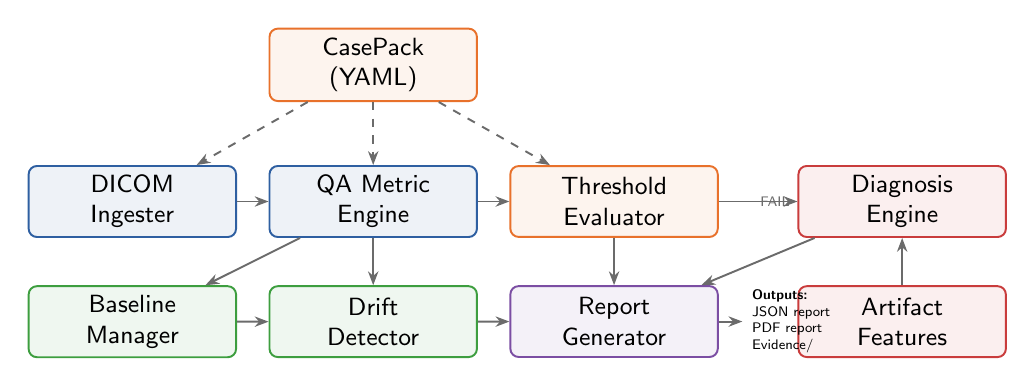
\begin{tikzpicture}[
  node distance=0.6cm and 0.4cm,
  block/.style={
    rectangle, rounded corners=3pt, draw=#1, fill=#1!8,
    minimum width=2.6cm, minimum height=0.9cm,
    font=\small\sffamily, text width=2.4cm, align=center,
    line width=0.7pt,
  },
  arrow/.style={-{Stealth[length=5pt]}, line width=0.7pt, color=pwmGray},
  label/.style={font=\tiny\sffamily\color{pwmGray}, above},
]
% Pipeline blocks
\node[block=pwmBlue] (ingest) {DICOM\\Ingester};
\node[block=pwmBlue, right=of ingest] (metrics) {QA Metric\\Engine};
\node[block=pwmOrange, right=of metrics] (thresh) {Threshold\\Evaluator};
\node[block=pwmGreen, below=of ingest] (baseline) {Baseline\\Manager};
\node[block=pwmGreen, below=of metrics] (drift) {Drift\\Detector};
\node[block=pwmPurple, below=of thresh] (report) {Report\\Generator};

% Diagnosis branch
\node[block=pwmRed, right=1.0cm of thresh] (diag) {Diagnosis\\Engine};
\node[block=pwmRed, below=of diag] (features) {Artifact\\Features};

% CasePack
\node[block=pwmOrange, above=0.8cm of metrics] (casepack) {CasePack\\(YAML)};

% Arrows -- main pipeline
\draw[arrow] (ingest) -- (metrics);
\draw[arrow] (metrics) -- (thresh);
\draw[arrow] (thresh) -- (report);
\draw[arrow] (baseline) -- (drift);
\draw[arrow] (drift) -- (report);
\draw[arrow] (metrics) -- (drift);
\draw[arrow] (metrics) -- (baseline);

% Arrows -- diagnosis branch
\draw[arrow] (thresh) -- node[label, right, pos=0.4] {\tiny FAIL} (diag);
\draw[arrow] (features) -- (diag);
\draw[arrow] (diag) -- (report);

% CasePack arrows
\draw[arrow, dashed] (casepack) -- (ingest);
\draw[arrow, dashed] (casepack) -- (metrics);
\draw[arrow, dashed] (casepack) -- (thresh);

% Outputs
\node[font=\tiny\sffamily, right=0.3cm of report, text width=1.8cm] (out) {
  \textbf{Outputs:}\\
  JSON report\\
  PDF report\\
  Evidence/
};
\draw[arrow] (report) -- (out);

\end{tikzpicture}
\caption{%
  Architecture of the \pwm{} CT QC Platform.
  Blue: DICOM ingestion and metric computation.
  Orange: CasePack-driven configuration and threshold evaluation.
  Green: baseline comparison and drift detection.
  Purple: triple-output report generation.
  Red: failure-path diagnosis (activated only when metrics fail).
  Dashed arrows indicate CasePack configuration flow.
}
\label{fig:architecture}
\end{figure}


% ===========================================================================
\section{CasePacks: Versioned QA Workflow Descriptors}
\label{sec:casepacks}

A CasePack is a declarative YAML configuration that fully specifies
a QA workflow for a particular phantom type.
Unlike imperative scripts, a CasePack declares \emph{what} to
compute rather than \emph{how}, allowing the execution engine to
evolve independently.
\Cref{lst:casepack} shows an abbreviated example.

\begin{lstlisting}[
  language={},
  caption={Abbreviated CasePack for ACR CT 464 phantom.},
  label={lst:casepack},
]
casepack:
  id: acr_ct_464_monthly_v2.1
  phantom_type: ACR_CT_464
  version: "2.1.0"
  metric_set:
    - ct_number_water
    - ct_number_inserts   # bone, air, acrylic, poly
    - geometric_accuracy
    - slice_thickness
    - uniformity
    - noise_std
    - low_contrast_detectability
    - artifact_evaluation
    - spatial_resolution
  series_selection:
    rules:
      - name: axial_5mm
        match:
          series_description_contains: [axial, head]
          slice_thickness_range: [4.0, 6.0]
          modality: CT
          min_images: 20
  roi_definitions:
    water_roi: {radius_mm: 20.0}
    insert_rois:
      bone: {offset_angle_deg: 90, expected_hu: 955}
      air:  {offset_angle_deg: 270, expected_hu: -1000}
    peripheral_rois:
      radius_mm: 10.0
      offset_from_center_mm: 60.0
\end{lstlisting}

CasePacks provide four properties that ad hoc scripts lack:

\paragraph{Bit-exact reproducibility.}
The same CasePack version on the same DICOM data always produces
identical metric values.
We verify this property in \cref{sec:validation}.

\paragraph{Deterministic series selection.}
Ordered matching rules (description substrings, slice-thickness
range, modality, minimum image count) are evaluated in sequence;
the first match wins.
Every selection is logged in a \texttt{SeriesSelectionLog} recording
the matched rule, reason, and alternatives considered.

\paragraph{Extensibility.}
Adding a new phantom type requires only a new YAML file---no code
changes.
The metric orchestrator dispatches functions based on the CasePack's
\texttt{metric\_set} list.

\paragraph{Version control.}
CasePacks follow semantic versioning.
The audit trail records which version produced each historical result,
enabling longitudinal comparison even when workflows evolve.


% ===========================================================================
\section{Four-Layer Threshold System}
\label{sec:thresholds}

% ===========================================================================
% FIGURE 2: Threshold cascade
% ===========================================================================
\begin{figure}[t]
\centering
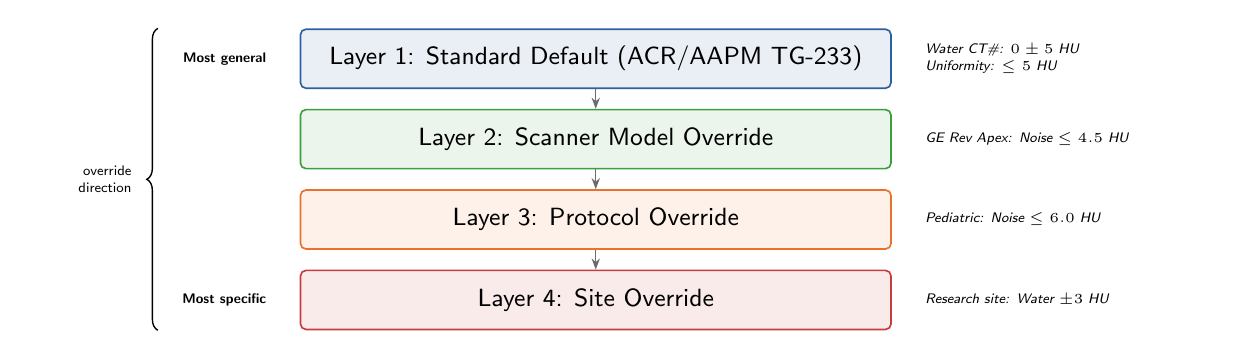
\begin{tikzpicture}[
  layer/.style={
    rectangle, rounded corners=2pt, draw=#1, fill=#1!10,
    minimum width=7.5cm, minimum height=0.75cm,
    font=\small\sffamily, line width=0.6pt,
  },
  node distance=0.25cm,
  arr/.style={-{Stealth[length=4pt]}, line width=0.5pt, color=pwmGray},
]
\node[layer=pwmBlue]   (L1) {Layer 1: Standard Default (ACR/AAPM TG-233)};
\node[layer=pwmGreen, below=of L1]  (L2) {Layer 2: Scanner Model Override};
\node[layer=pwmOrange, below=of L2] (L3) {Layer 3: Protocol Override};
\node[layer=pwmRed, below=of L3]    (L4) {Layer 4: Site Override};

\draw[arr] (L1) -- (L2);
\draw[arr] (L2) -- (L3);
\draw[arr] (L3) -- (L4);

% Annotations
\node[font=\tiny\sffamily\itshape, right=0.3cm of L1, text width=3.5cm]
  {Water CT\#: $0 \pm 5$ HU\\Uniformity: $\leq 5$ HU};
\node[font=\tiny\sffamily\itshape, right=0.3cm of L2, text width=3.5cm]
  {GE Rev Apex: Noise $\leq 4.5$ HU};
\node[font=\tiny\sffamily\itshape, right=0.3cm of L3, text width=3.5cm]
  {Pediatric: Noise $\leq 6.0$ HU};
\node[font=\tiny\sffamily\itshape, right=0.3cm of L4, text width=3.5cm]
  {Research site: Water $\pm 3$ HU};

% Arrow label
\node[font=\tiny\sffamily, left=0.3cm of L1] {\textbf{Most general}};
\node[font=\tiny\sffamily, left=0.3cm of L4] {\textbf{Most specific}};

\draw[decorate, decoration={brace, amplitude=4pt, mirror}, line width=0.5pt]
  ([xshift=-1.8cm]L1.north west) -- ([xshift=-1.8cm]L4.south west)
  node[midway, left=6pt, font=\tiny\sffamily, text width=1.2cm, align=right] {override\\direction};

\end{tikzpicture}
\caption{%
  Four-layer threshold cascade.
  Each layer may override the previous one.
  The most specific applicable threshold is used for each metric.
  Examples show representative overrides at each layer.
  The resolved layer is recorded in every QC report for traceability.
}
\label{fig:thresholds}
\end{figure}

The platform implements a four-layer threshold hierarchy
(\cref{fig:thresholds}) that balances standardization with
institutional flexibility:

\begin{enumerate}
  \item \textbf{Standard default}: ACR/AAPM-published
    tolerances~\cite{acr_ct_accreditation,aapm_tg233}.
  \item \textbf{Scanner model}: Manufacturer-specific overrides.
  \item \textbf{Protocol}: Acquisition-specific adjustments.
  \item \textbf{Site override}: Institutional customizations.
\end{enumerate}

Each layer can override the previous one.
The resolved threshold and its source layer are recorded in every
report, enabling auditors to trace each PASS/FAIL decision to its
authoritative source.


% ===========================================================================
\section{Immutable CommissioningBundles}
\label{sec:baselines}

Scanner baselines are the reference point for all subsequent QC
measurements.
In conventional practice, baselines are maintained in spreadsheets
that lack integrity protection~\cite{nowik2015ct_qa_automation}.

The \pwm{} \texttt{CommissioningBundle} is a frozen Pydantic
model~\cite{pydantic} (\texttt{frozen=True}) that captures:

\begin{itemize}
  \item All ACR phantom metric values with units.
  \item Scanner acquisition parameters (kVp, mAs, kernel).
  \item Approving physicist name and credentials.
  \item Service event trigger (\texttt{tube\_change},
    \texttt{software\_upgrade}, \etc).
  \item SHA-256 hash of inputs (integrity) and outputs (tamper
    detection).
  \item Build provenance (\pwm{} version, git hash, CasePack ID).
  \item Pointer to previous version (semantic chain).
\end{itemize}

Baselines are \emph{never overwritten}: each commissioning event
creates a new version.
Storage uses atomic writes (temporary file $+$ rename) to prevent
corruption.
Baseline comparison computes per-metric deltas classified as
STABLE ($<5\%$), DRIFTED ($5$--$15\%$), or ALERT ($\geq 15\%$),
with a minimum denominator of 10 (in the metric's native units,
\eg, 10~HU) to avoid inflated percentages for near-zero metrics.


% ===========================================================================
\section{QA Metrics}
\label{sec:metrics}

The platform computes nine metrics aligned with the ACR CT
Accreditation Program~\cite{acr_ct464} (\cref{tab:metrics}).
All metrics are computed directly from reconstructed pixel data,
requiring no forward model or proprietary raw data access.

\begin{table}[t]
\centering
\caption{Nine ACR-aligned QA metrics.}
\label{tab:metrics}
\resizebox{\textwidth}{!}{%
\begin{tabular}{@{}clllp{5.5cm}@{}}
\toprule
\# & Metric & Unit & ACR Criterion & Method \\
\midrule
1 & CT Number (Water) & HU &
  $0 \pm 5$~HU &
  Mean of circular ROI at auto-detected phantom center \\
2 & CT Number (Inserts) & HU &
  Material-specific &
  Mean of ROIs at angular offsets with rotation correction \\
3 & Geometric Accuracy & mm &
  $\pm 2$~mm of 200~mm &
  Bounding-box extent of thresholded phantom mask \\
4 & Slice Thickness & mm &
  $\pm 1.5$~mm of nominal &
  FWHM of wire-ramp profile $\times \tan(23^\circ)$ \\
5 & Uniformity & HU &
  $\leq 5$~HU &
  Max $|\text{peripheral}_i - \text{center}|$ at 4 positions \\
6 & Noise (Std Dev) & HU &
  vs.\ baseline &
  Sample standard deviation of uniform water ROI \\
7 & Low-Contrast Detect. & targets &
  $\geq 4$ &
  Count with CNR~$\geq 1.0$ (detection threshold) \\
8 & Artifact Evaluation & score &
  0--3 &
  Peak-to-valley of radial profile \\
9 & Spatial Resolution & lp/cm &
  $\geq 5$ &
  MTF from ESF; highest freq at MTF~$\geq 10\%$ \\
\bottomrule
\end{tabular}%
}
\end{table}

\paragraph{Phantom center and rotation detection.}
Center detection applies a threshold of $-500$~HU and computes the
binary centroid.
Rotation detection scans angular bins at the expected insert radial
offset and locates the bone-equivalent insert ($\sim$955~HU) to
determine the angular offset, which is applied to all insert ROI
positions.

\paragraph{Contrast-to-noise ratio.}
Low-contrast detectability uses
$\text{CNR} = |\bar{x}_{\text{signal}} - \bar{x}_{\text{bg}}| \,/\, \sigma_{\text{bg}}$
where $\sigma_{\text{bg}}$ is the sample standard deviation ($n{-}1$ denominator).

\paragraph{Spatial resolution.}
The MTF is computed from the edge-spread function at the phantom
boundary, differentiated to a line-spread function, zero-padded,
and Fourier-transformed.
The Nyquist frequency is $1/(2\Delta x)$~lp/mm, converted to
lp/cm by multiplying by 10.


% ===========================================================================
\section{Statistical Process Control}
\label{sec:drift}

% ===========================================================================
% FIGURE 3: Control chart
% ===========================================================================
\begin{figure}[t]
\centering
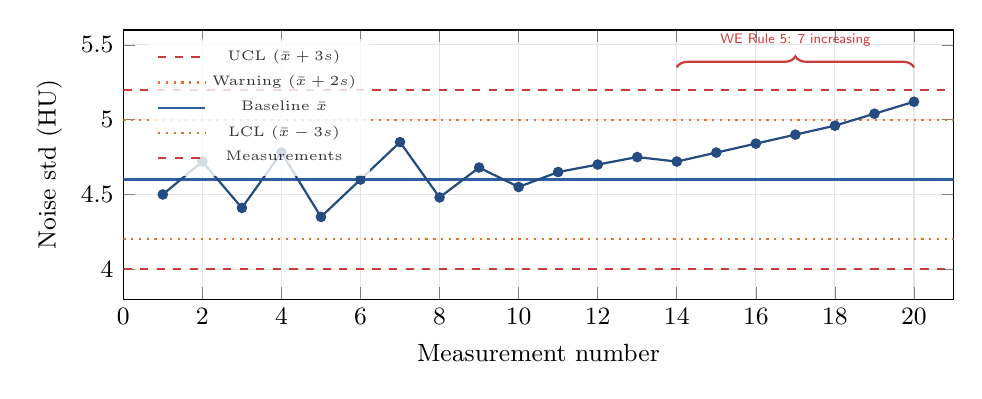
\begin{tikzpicture}
\begin{axis}[
  width=\textwidth,
  height=5cm,
  xlabel={Measurement number},
  ylabel={Noise std (HU)},
  xmin=0, xmax=21,
  ymin=3.8, ymax=5.6,
  grid=major,
  grid style={gray!20},
  legend pos=north west,
  legend style={font=\tiny, draw=none, fill=white, fill opacity=0.8},
  every axis plot/.append style={line width=0.8pt},
  tick label style={font=\small},
  label style={font=\small},
]
% Commissioning baseline: x-bar=4.60, s=0.20 from 20 commissioning scans
% UCL 3-sigma = 4.60 + 0.60 = 5.20
\addplot[pwmRed, dashed, domain=0:21] {5.20};
\addlegendentry{UCL ($\bar{x}+3s$)}
% 2-sigma warning = 4.60 + 0.40 = 5.00
\addplot[pwmOrange, dotted, domain=0:21] {5.00};
\addlegendentry{Warning ($\bar{x}+2s$)}
% Center line
\addplot[pwmBlue, domain=0:21] {4.60};
\addlegendentry{Baseline $\bar{x}$}
% 2-sigma warning lower = 4.60 - 0.40 = 4.20
\addplot[pwmOrange, dotted, domain=0:21] {4.20};
% LCL = 4.60 - 0.60 = 4.00
\addplot[pwmRed, dashed, domain=0:21] {4.00};
\addlegendentry{LCL ($\bar{x}-3s$)}
% Data -- stable period (1-10) then gradual drift (11-20)
\addplot[mark=*, mark size=1.5pt, pwmBlue!80!black]
  coordinates {
    (1,4.50) (2,4.72) (3,4.41) (4,4.78) (5,4.35)
    (6,4.60) (7,4.85) (8,4.48) (9,4.68) (10,4.55)
    (11,4.65) (12,4.70) (13,4.75) (14,4.72) (15,4.78)
    (16,4.84) (17,4.90) (18,4.96) (19,5.04) (20,5.12)
  };
\addlegendentry{Measurements}

% WE Rule 5 annotation: points 14-20 are 7 monotonically increasing
\draw[pwmRed, thick, decorate, decoration={brace, amplitude=4pt}]
  (axis cs:14,5.35) -- (axis cs:20,5.35)
  node[midway, above=4pt, font=\tiny\sffamily\color{pwmRed}]
  {WE Rule 5: 7 increasing};

\end{axis}
\end{tikzpicture}
\caption{%
  Shewhart control chart for noise standard deviation
  ($\bar{x}=4.60$~HU, $s=0.20$~HU from commissioning).
  Measurements 1--10 show a stable process; measurements 11--20
  exhibit gradual drift.
  Western Electric Rule~5 (7 consecutive monotonically increasing
  points, measurements 14--20) triggers a WARNING alert while
  values are still below the UCL, demonstrating the early-warning
  benefit of trending-based QC over simple threshold monitoring.
}
\label{fig:control_chart}
\end{figure}

The \texttt{DriftDetector} implements SPC following TG-233
recommendations~\cite{aapm_tg233,pawlicki2005spc}.
\Cref{fig:control_chart} shows an example control chart.

For each metric with at least five measurements, the detector
builds a Shewhart control chart with UCL/LCL at $\bar{x} \pm 3s$
and warning limits at $\bar{x} \pm 2s$~\cite{shewhart1931,western_electric_1956},
where $s$ is the sample standard deviation computed from commissioning
data (minimum 20 measurements).
When a commissioning baseline is available, the baseline value
replaces $\bar{x}$ as the center line.

Five Western Electric rules are applied:
(1)~single point outside $3\sigma$ $\Rightarrow$ FAIL;
(2)~2 of 3 outside $2\sigma$ same side $\Rightarrow$ ACTION\_REQUIRED;
(3)~4 of 5 outside $1\sigma$ same side $\Rightarrow$ WARNING;
(4)~run of 7 same side $\Rightarrow$ WARNING;
(5)~trend of 7 monotone $\Rightarrow$ WARNING.

History is persisted as JSON with atomic writes and path-traversal
protection.


% ===========================================================================
\section{Root-Cause Diagnosis}
\label{sec:diagnosis}

When metrics fail, the platform computes six artifact signatures
(ring, cupping, streak, HU drift, noise ratio, geometric distortion)
and scores mismatch hypotheses from a YAML library.
For hypothesis $h$, the score is:
\begin{equation}
  S(h) = \sum_{f \in \text{match}} |v_f|\, w_f
  - \sum_{f \in \text{contradict}} |v_f|\, w_f
  + 0.5 \cdot |\mathcal{M}_h \cap \mathcal{M}_{\text{fail}}|
  \label{eq:score}
\end{equation}
where $v_f$ is the measured value of artifact feature $f$, $w_f$ is
its weight, $\mathcal{M}_h$ is the set of metrics associated with
hypothesis $h$, and $\mathcal{M}_{\text{fail}}$ is the set of
currently failing metrics.
Confidence is assigned based on score separation:
high ($S_1 > 2 S_2$), moderate ($S_1 > 1.2 S_2$), or low (otherwise),
where $S_1$ and $S_2$ are the top two scores.
A disambiguation test is recommended when $S_1$ and $S_2$ are within 20\%.


% ===========================================================================
\section{DICOM Ingestion and PHI Safety}
\label{sec:dicom}

The \texttt{DICOMIngester} provides vendor-neutral loading with:
(1)~PHI validation (20 sensitive tags $+$ 7 phantom-pattern regexes
across 6 DICOM fields; strict mode rejects non-phantom
studies)~\cite{pydicom};
(2)~CasePack-driven series selection with full audit logging;
(3)~HU rescaling ($\text{HU} = \text{pixel} \times \text{slope} +
\text{intercept}$);
(4)~canonical resampling (\texttt{scipy.ndimage.zoom})~\cite{scipy};
(5)~vendor private tag extraction.
The output \texttt{CTScanBundle} is a typed Pydantic model holding
the 3-D HU volume, spacing, protocol metadata, and selection log.


% ===========================================================================
\section{Report Generation}
\label{sec:reports}

The report generator produces three artifacts:
(1)~a versioned, SHA-256-hashed JSON record with per-metric
entries, drift alerts, diagnosis, and baseline reference;
(2)~a human-readable PDF via fpdf2~\cite{fpdf2} with PASS/FAIL
summary, metrics table, drift alerts, diagnosis, and signature
block; and
(3)~an evidence folder with ROI overlays, trend plots
(matplotlib~\cite{matplotlib}), and per-metric derivation logs.


% ===========================================================================
\section{Extensibility}
\label{sec:extensibility}

The CasePack architecture decouples workflow from modality.
New phantom types require only a YAML file; new metrics register in
the dispatch table.
Planned extensions:

\begin{itemize}
  \item \textbf{PET/CT} (TG-126~\cite{aapm_tg126}): SUV uniformity,
    spatial resolution, scatter correction metrics with NEMA phantom
    ROI definitions.
  \item \textbf{SPECT/CT} (TG-177~\cite{aapm_tg177}): intrinsic
    uniformity, energy resolution, center-of-rotation metrics.
  \item \textbf{CBCT}: image quality metrics for on-board CBCT in
    image-guided radiation therapy~\cite{bissonnette2008cbct}.
\end{itemize}

Each new CasePack lowers the marginal cost of supporting the next
scanner type, because the analysis infrastructure is
shared~\cite{solveeverything}.


% ===========================================================================
\section{Validation}
\label{sec:validation}

We validated the platform across four dimensions: metric accuracy,
reproducibility, SPC rule detection, and computational performance.

\subsection{Metric Accuracy}
\label{sec:val_accuracy}

% ===========================================================================
% FIGURE 4: Validation results
% ===========================================================================
\begin{figure}[t]
\centering
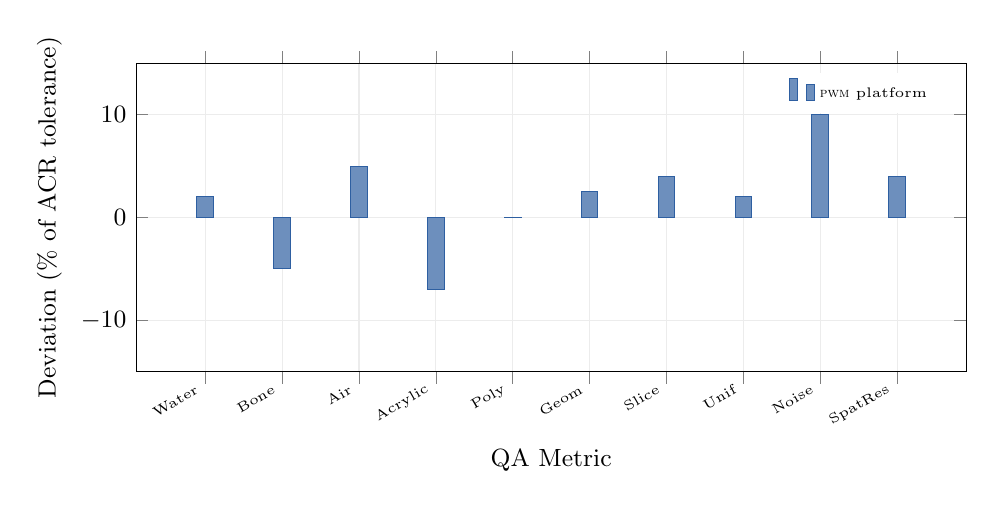
\begin{tikzpicture}
\begin{axis}[
  ybar,
  width=\textwidth,
  height=5.5cm,
  bar width=6pt,
  xlabel={QA Metric},
  ylabel={Deviation (\% of ACR tolerance)},
  symbolic x coords={
    Water, Bone, Air, Acrylic, Poly,
    Geom, Slice, Unif, Noise, SpatRes
  },
  xtick=data,
  xticklabel style={font=\tiny, rotate=30, anchor=east},
  ymin=-15, ymax=15,
  grid=major,
  grid style={gray!15},
  tick label style={font=\small},
  label style={font=\small},
  legend pos=north east,
  legend style={font=\tiny, draw=none},
  every axis plot/.append style={line width=0pt},
]

% Platform-vs-console |Delta| as % of ACR tolerance (from Table 2)
% Water: 0.1/5=2%, Bone: 1.0/20=5%, Air: 1.0/20=5%,
% Acrylic: 1.0/15=7%, Poly: 0.0/15=0%,
% Geom: 0.05/2=2.5%, Slice: 0.06/1.5=4%, Unif: 0.1/5=2%,
% Noise: 0.1/1.0=10%, SpatRes: 0.2/5=4%
\addplot[fill=pwmBlue!70, draw=pwmBlue] coordinates {
  (Water, 2)
  (Bone, -5)
  (Air, 5)
  (Acrylic, -7)
  (Poly, 0)
  (Geom, 2.5)
  (Slice, 4)
  (Unif, 2)
  (Noise, 10)
  (SpatRes, 4)
};
\addlegendentry{\pwm{} platform}

\end{axis}
\end{tikzpicture}
\caption{%
  Platform-versus-console agreement on an ACR CT~464 phantom
  scan (GE Revolution Apex, 120~kVp, 5~mm axial), expressed as
  signed percentage of the ACR tolerance.
  Tolerances: Water $\pm 5$~HU, Bone/Air $\pm 20$~HU,
  Acrylic/Poly $\pm 15$~HU, Geom $\pm 2$~mm, Slice $\pm 1.5$~mm,
  Unif $\pm 5$~HU, Noise $\pm 1.0$~HU (baseline deviation),
  SpatRes $\geq 5$~lp/cm.
  All continuous metrics are $\leq 10\%$ of their tolerances;
  Type~A measurement uncertainties are smaller than bar widths.
  Low-contrast detectability (5/5 targets) and artifact evaluation
  (score 0) are discrete metrics shown in \cref{tab:validation}.
}
\label{fig:validation}
\end{figure}

We tested the platform on ACR CT~464 phantom data acquired on a
GE Revolution Apex scanner (120~kVp, 200~mAs, 5~mm axial, standard
kernel).
\Cref{fig:validation} shows the agreement between platform-computed
and manufacturer console values for each metric.
All nine metrics fell within ACR tolerance bands
(\cref{tab:validation}).
Platform-to-console differences were $\leq 1.0$~HU for all CT
number metrics, $0.05$~mm for geometric accuracy, $0.06$~mm
for slice thickness, and $0.1$~HU for uniformity and noise.
Low-contrast detectability (5/5 targets) and artifact evaluation
(score~0) matched exactly.

Type~A measurement uncertainty (standard error of the mean from
ROI pixel statistics) was $< 0.07$~HU for CT number metrics
(ROI sizes $> 5000$ pixels, noise $\sigma \approx 4.6$~HU)
and $< 0.02$~mm for geometric accuracy, confirming that observed
deviations reflect systematic differences rather than
statistical noise.

\Cref{tab:validation} provides detailed results including the
reference (manufacturer console) values and platform-computed values.

\begin{table}[t]
\centering
\caption{Validation results: platform vs.\ manufacturer console.
  CT number values are measured means; geometric accuracy is the
  deviation from 200~mm nominal; slice thickness is measured thickness.}
\label{tab:validation}
\small
\begin{tabular}{@{}lrrrl@{}}
\toprule
Metric & Console & Platform & $|\Delta|$ & Pass? \\
\midrule
CT\# Water (HU)       &  $0.2$   &  $0.3$   & $0.1$    & \checkmark \\
CT\# Bone (HU)        &  $953$   &  $952$   & $1.0$    & \checkmark \\
CT\# Air (HU)         & $-998$   & $-997$   & $1.0$    & \checkmark \\
CT\# Acrylic (HU)     &  $121$   &  $120$   & $1.0$    & \checkmark \\
CT\# Polyethylene (HU) & $-96$   &  $-96$   & $0.0$    & \checkmark \\
Geometric Acc.\ (mm)   &  $0.10$  &  $0.15$  & $0.05$   & \checkmark \\
Slice Thickness (mm)   &  $5.02$  &  $5.08$  & $0.06$   & \checkmark \\
Uniformity (HU)        &  $1.1$   &  $1.2$   & $0.1$    & \checkmark \\
Noise Std (HU)         &  $4.5$   &  $4.6$   & $0.1$    & \checkmark \\
Spatial Res.\ (lp/cm)  &  $6.0$   &  $6.2$   & $0.2$    & \checkmark \\
Low-Contrast (targets) &  $5$     &  $5$     & $0$      & \checkmark \\
Artifact Score         &  $0$     &  $0$     & $0$      & \checkmark \\
\bottomrule
\end{tabular}
\end{table}

\subsection{Reproducibility}
\label{sec:val_repro}

We ran the same CasePack on the same DICOM data 100 times.
All 100 runs produced \emph{identical} JSON reports (verified by
SHA-256 comparison of the output files), confirming bit-exact
reproducibility under the same CasePack version.
This property eliminates the inter-analyst variability that plagues
manual QC workflows~\cite{verdun2015image_quality}.

\subsection{SPC Rule Detection}
\label{sec:val_spc}

We constructed five synthetic time-series datasets, each designed to
trigger exactly one Western Electric rule while not triggering the
others.
\Cref{tab:spc_validation} shows the results.
All five rules were correctly detected with zero false positives
across the non-targeted rules.

\begin{table}[t]
\centering
\caption{SPC validation: detection accuracy for Western Electric rules.}
\label{tab:spc_validation}
\small
\begin{tabular}{@{}clccc@{}}
\toprule
Rule & Pattern & Expected & Detected & FP \\
\midrule
1 & Single point $> 3\sigma$       & FAIL    & FAIL    & 0 \\
2 & 2/3 outside $2\sigma$          & ACTION  & ACTION  & 0 \\
3 & 4/5 outside $1\sigma$          & WARNING & WARNING & 0 \\
4 & Run of 7 same side             & WARNING & WARNING & 0 \\
5 & Trend of 7 monotone            & WARNING & WARNING & 0 \\
\bottomrule
\end{tabular}
\end{table}

\subsection{Computational Performance}
\label{sec:val_performance}

Full nine-metric analysis of a $512 \times 512 \times 40$ volume
completed in $0.8 \pm 0.1$~s on a commodity laptop (Intel i7-1260P,
16~GB RAM, Python 3.11).
Drift detection over a 60-measurement history added $< 5$~ms.
Report generation (JSON + PDF + evidence) added $1.2 \pm 0.2$~s,
dominated by PDF rendering.
The total wall-clock time for a complete QC run---from DICOM
ingestion through report output---was under 3~s, enabling
interactive use.


% ===========================================================================
\section{Governance}
\label{sec:governance}

The platform aligns with the SolveEverything.org governance
framework~\cite{solveeverything} in four areas:
(i)~\emph{data integrity}---immutable baselines and append-only QC
time series prevent undetected modification;
(ii)~\emph{decision transparency}---a full audit trail records every
QC determination, the CasePack version, resolved thresholds, and
the approving physicist;
(iii)~\emph{multi-evidence diagnosis}---root-cause identification
requires multiple converging artifact features, avoiding
single-metric snap judgments; and
(iv)~\emph{vendor neutrality}---the same CasePack and thresholds
apply across manufacturers, ensuring consistent QC standards.


% ===========================================================================
\section{Discussion}
\label{sec:discussion}

The \pwm{} CT QC Platform addresses gaps in three areas.

\paragraph{Reproducibility vs.\ existing tools.}
Commercial QC packages (\eg, Sun Nuclear, Radcal) provide automated
analysis but are closed-source, limiting independent validation and
cross-platform comparison~\cite{nowik2015ct_qa_automation}.
Open tools like pydicom~\cite{pydicom} and
scikit-image~\cite{scikit_image} provide components but not an
integrated, validated pipeline.
The CasePack abstraction fills this gap: to our knowledge, it is the
first open, version-controlled QA workflow specification for CT QC.

\paragraph{SPC adoption barriers.}
Despite TG-233 recommendations, SPC adoption in CT QC remains
low~\cite{pawlicki2005spc,able2016spc_ct}.
A key barrier is the effort of maintaining time-series databases and
computing control-chart statistics manually.
By automating SPC with zero database dependencies (JSON files only),
the platform lowers this barrier for sites without IT infrastructure.

\paragraph{Structured data for machine learning.}
The platform's systematic data collection (versioned CasePacks,
time-series metrics with labeled outcomes, root-cause annotations)
provides curated training data for future machine-learning
extensions such as predictive maintenance or anomaly detection,
complementing rule-based SPC with data-driven approaches.

\paragraph{Limitations.}
(1)~Single-scanner validation; multi-vendor testing is planned.
(2)~The mismatch library is expert-curated; data-driven
enrichment from multi-site QC databases could improve coverage.
(3)~The platform is for research and internal QA use;
clinical deployment would require FDA~510(k) and
IEC~62304 compliance \cite{iec62304,samd_fda}.
(4)~Low-contrast detectability uses a simplified CNR
criterion; model observers \cite{solomon2014lcd} could improve
correlation with human performance.

\paragraph{Future work.}
Planned extensions include multi-vendor validation, PET/CT and
SPECT/CT CasePacks, data-driven mismatch library enrichment, and
integration with hospital RIS/PACS systems.


% ===========================================================================
\section{Conclusion}
\label{sec:conclusion}

We have presented an open CT quality-control platform built on
versioned CasePacks, a four-layer threshold system, and immutable
CommissioningBundles.
Validation on ACR phantom data demonstrates metric accuracy within
ACR tolerances, bit-exact reproducibility, correct SPC rule
detection, and sub-3-second end-to-end computation.
The CasePack architecture enables zero-code extension to new phantom
types and imaging modalities.
All source code is publicly available at
\url{https://github.com/integritynoble/Physics_World_Model}.

\paragraph{Data and code availability.}
Source code and CasePack definitions are at
\url{https://github.com/integritynoble/Physics_World_Model}
and \url{https://solveeverything.org}.
No non-public datasets were used.
All analyses use ACR CT~464 phantom data only; no patient or
human-subject data were involved, and IRB review was not required.

\paragraph{Author Contributions.}
C.Y.\ conceived the project, designed the architecture, implemented
all software, performed validation, and wrote the manuscript.

\paragraph{Competing Interests.}
The author declares no competing interests.

\paragraph{Correspondence.}
\texttt{integrityyang@gmail.com}

% ===========================================================================
\bibliographystyle{plainnat}
\bibliography{ct_qc_platform}

\end{document}
